\subsection{Frozen v3 policy holdout: exact radix evaluation}
\label{sec:pr-engine-results}
Each platform completed all 924 tasks on the same 308 series in 17 families,
with $L=30$ primary, $L=100$ secondary, and $L=300$ a stress regime.
Each task evaluates the three frozen model score vectors and returns the best-PR model set, retaining numerical ties.
Times include whole-task preparation and use the median of three repetitions.
The maximum absolute PR discrepancy from the comparison-sort sparse PR reference was
$1.554\times 10^{-15}$ on Mac and $1.332\times 10^{-15}$ on Linux.
These are numerical agreement checks for the pinned target.

The frozen exact-radix decision at $L=30$ is Mac: \textbf{PASS}; Linux: \textbf{PASS}.
It requires both the geometric-mean and aggregate-ratio lower confidence bounds
to exceed one against every one of the five frozen controls, together with correctness.
Klein and Benchopt comparisons are descriptive and are outside this decision.
Table~\ref{tab:radix-primary} retains every primary control and both external implementations.

All ratios are comparator time divided by exact sparse-radix PR time; values above one favor radix PR.
Brackets contain audited 95\% family-cluster bootstrap intervals (2000 resamples).
The aggregate ratio divides sums of per-case median times; it is not an observed batch wall time.
Intervals describe variation across families, not uncertainty in three timing repetitions.
F/S/T counts cases where radix PR is faster/slower/tied. Decisions use unrounded bounds.

\begin{table}[tbp]
\centering\small
\setlength{\tabcolsep}{3pt}
\caption{Primary $L=30$: all 308 cases per platform. $\dagger$ marks the five frozen decision controls. R+P methods compute both ROC and PR; the others compute PR only. Dense direct and dense nearest use comparison sorting unless labelled radix.}
\label{tab:radix-primary}
\resizebox{\linewidth}{!}{%
\begin{tabular}{llrrrr}
\toprule
Platform & Comparator & Median & Geomean [CI] & Aggregate [CI] & F/S/T \\
\midrule
Mac & Sparse comparison$^{\dagger}$ & 1.774 & 1.620 [1.421, 1.920] & 1.960 [1.511, 2.323] & 271/37/0 \\
Mac & Dense direct$^{\dagger}$ & 3.331 & 3.160 [2.772, 3.506] & 4.255 [3.349, 5.112] & 306/2/0 \\
Mac & Dense nearest (R+P)$^{\dagger}$ & 5.050 & 4.840 [4.356, 5.368] & 6.140 [4.974, 7.181] & 308/0/0 \\
Mac & Dense direct radix$^{\dagger}$ & 2.677 & 2.617 [2.318, 2.870] & 3.595 [2.752, 4.514] & 303/5/0 \\
Mac & Dense nearest radix$^{\dagger}$ & 2.599 & 2.519 [2.297, 2.726] & 3.298 [2.624, 3.980] & 307/1/0 \\
Mac & Klein fast-VUS & 20.925 & 22.360 [19.764, 24.238] & 19.450 [17.910, 20.623] & 308/0/0 \\
Mac & Benchopt (R+P) & 35.420 & 37.572 [34.754, 41.101] & 37.990 [34.728, 42.965] & 308/0/0 \\
\midrule
Linux & Sparse comparison$^{\dagger}$ & 1.987 & 1.916 [1.839, 2.013] & 1.955 [1.745, 2.095] & 304/4/0 \\
Linux & Dense direct$^{\dagger}$ & 4.894 & 4.161 [3.170, 5.008] & 5.385 [4.241, 6.191] & 308/0/0 \\
Linux & Dense nearest (R+P)$^{\dagger}$ & 6.917 & 5.890 [4.639, 6.923] & 7.214 [5.688, 8.187] & 308/0/0 \\
Linux & Dense direct radix$^{\dagger}$ & 4.419 & 3.756 [2.904, 4.486] & 4.708 [3.794, 5.276] & 308/0/0 \\
Linux & Dense nearest radix$^{\dagger}$ & 4.791 & 4.047 [3.142, 4.821] & 5.010 [3.933, 5.643] & 306/2/0 \\
Linux & Klein fast-VUS & 14.538 & 13.814 [11.639, 15.930] & 11.232 [10.034, 12.514] & 308/0/0 \\
Linux & Benchopt (R+P) & 21.493 & 20.973 [18.481, 23.617] & 22.991 [19.193, 30.937] & 308/0/0 \\
\bottomrule
\end{tabular}}
\end{table}

\paragraph{Secondary and stress regimes.}
Table~\ref{tab:radix-secondary} gives both matched PR-only radix dense controls at $L=100$ and $L=300$.
These controls share fixed-width score ordering with sparse radix and retain full dense width sweeps.
Their ratios assess the support-event reduction after matching the ranking implementation.
The full bound reports retain every other comparator, family effect, and slower case at each width.

\begin{table}[tbp]
\centering\small
\setlength{\tabcolsep}{3pt}
\caption{Secondary and stress widths: all 308 cases per row, matched PR-only controls. Ratio direction and intervals follow Table~\ref{tab:radix-primary}.}
\label{tab:radix-secondary}
\resizebox{\linewidth}{!}{%
\begin{tabular}{lllrrrr}
\toprule
Platform & $L$ & Comparator & Median & Geomean [CI] & Aggregate [CI] & F/S/T \\
\midrule
Mac & 100 & Dense direct radix & 5.110 & 4.834 [3.728, 5.802] & 6.874 [4.488, 8.943] & 307/1/0 \\
Mac & 100 & Dense nearest radix & 4.637 & 4.551 [3.602, 5.370] & 6.096 [4.117, 7.577] & 305/3/0 \\
Mac & 300 & Dense direct radix & 6.916 & 6.534 [4.259, 8.903] & 8.850 [5.163, 12.681] & 308/0/0 \\
Mac & 300 & Dense nearest radix & 6.294 & 6.000 [3.902, 8.163] & 7.892 [4.670, 11.080] & 300/8/0 \\
Linux & 100 & Dense direct radix & 7.465 & 6.666 [4.438, 8.952] & 8.220 [5.435, 10.714] & 308/0/0 \\
Linux & 100 & Dense nearest radix & 7.919 & 6.975 [4.574, 9.447] & 8.543 [5.360, 11.345] & 302/6/0 \\
Linux & 300 & Dense direct radix & 7.612 & 7.360 [4.333, 10.986] & 8.808 [5.506, 13.079] & 308/0/0 \\
Linux & 300 & Dense nearest radix & 8.103 & 7.426 [4.155, 11.417] & 8.943 [5.047, 13.692] & 295/13/0 \\
\bottomrule
\end{tabular}}
\end{table}

\paragraph{Post-protocol descriptive PR-only oracle.}
For each case, the oracle selects the fastest of comparison-based sparse PR, direct dense PR,
Klein PR, direct dense radix PR, and nearest-interval dense radix PR.
Paired ROC+PR methods and adaptive racers are excluded from this PR-only exhaustive set.
Table~\ref{tab:radix-oracle} and Figure~\ref{fig:radix-oracle} retain every case and loss.
No confidence interval is assigned to this retrospective minimum, and it changes no frozen decision.

\begin{table}[tbp]
\centering\small
\setlength{\tabcolsep}{3pt}
\caption{Descriptive PR-only oracle / exact sparse-radix ratios; no confidence intervals. Minimum retains the slowest relative radix case.}
\label{tab:radix-oracle}
\resizebox{\linewidth}{!}{%
\begin{tabular}{llrrrrr}
\toprule
Platform & $L$ & Median & Geomean & Aggregate & F/S/T & Minimum \\
\midrule
Mac & 30 & 1.709 & 1.582 & 1.924 & 268/40/0 & 0.531 \\
Mac & 100 & 1.557 & 1.500 & 1.734 & 286/22/0 & 0.618 \\
Mac & 300 & 1.278 & 1.293 & 1.375 & 285/23/0 & 0.610 \\
Linux & 30 & 1.986 & 1.879 & 1.928 & 302/6/0 & 0.807 \\
Linux & 100 & 1.715 & 1.655 & 1.612 & 301/7/0 & 0.815 \\
Linux & 300 & 1.275 & 1.309 & 1.235 & 294/14/0 & 0.770 \\
\bottomrule
\end{tabular}}
\end{table}

\begin{figure}[tbp]
\centering
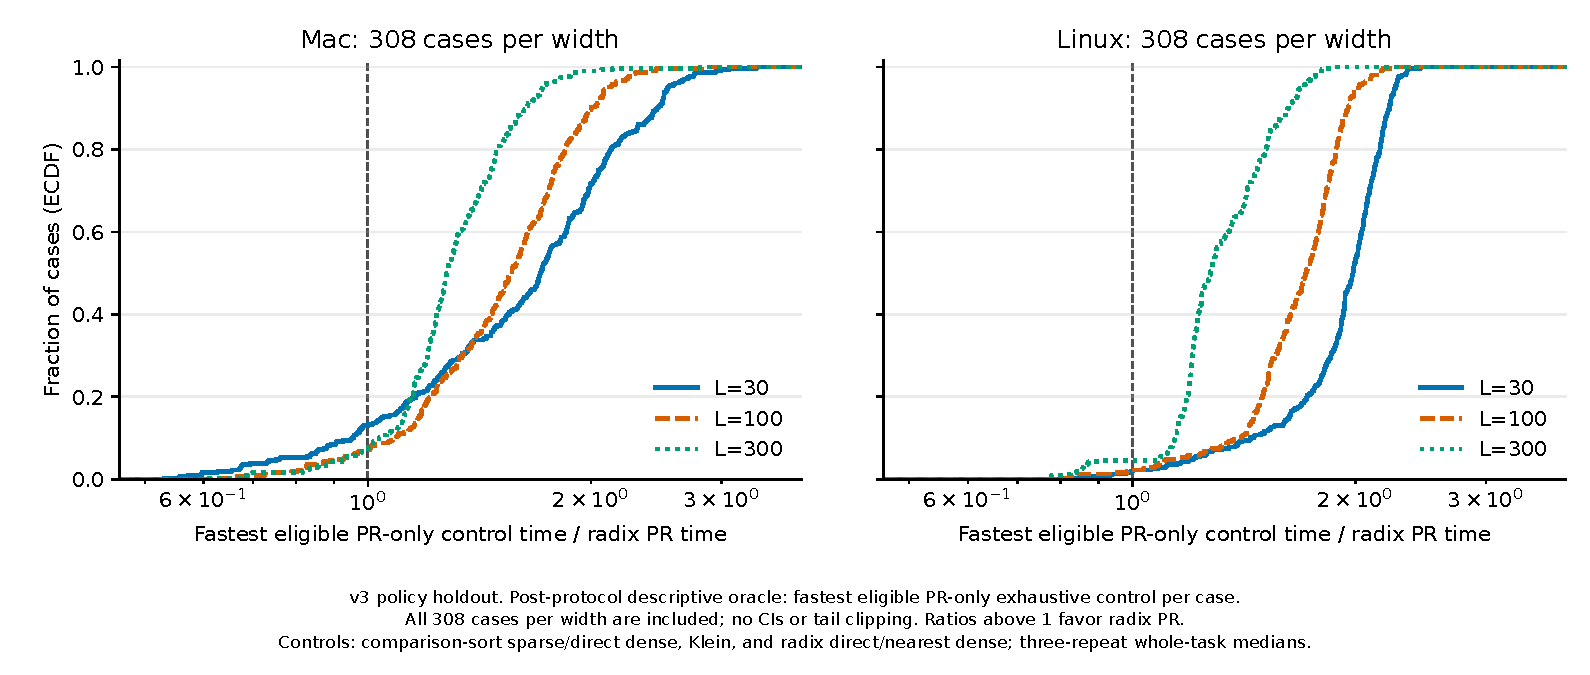
\includegraphics[width=\linewidth]{figures/pr-only-oracle-ecdf.pdf}
\caption{Post-protocol oracle ECDFs for the v3 policy holdout: all 308 cases at each width on each platform, without tail clipping. The horizontal coordinate is the fastest eligible exhaustive PR-only control's whole-task case median divided by exact sparse-radix PR time. Values above one favor radix PR. The five eligible controls are specified in the text; no oracle confidence intervals are computed.}
\label{fig:radix-oracle}
\end{figure}

\paragraph{Separate racing decisions and scope.}
The frozen comparison-order racing decision at $L=30$ is Mac \textbf{FAIL}, Linux \textbf{FAIL}; the separate radix-order racing decision is Mac \textbf{FAIL}, Linux \textbf{FAIL}.
The first requires both interval lower bounds above one against comparison-based sparse PR, direct dense PR, and exact radix PR;
the second additionally requires this against both matched dense radix PR controls.
These decisions include preparation, adaptive queries, and exact completion in each measured task.
Racing outcomes are separate from the exact-radix decision, and failed criteria remain reported.
The v2 development runs remain historical development evidence and are not pooled with this holdout.
Platforms are summarized separately: no cross-run timing pooling is performed.
The Mac was not isolated: its starting snapshot shows an unrelated Python worker near 100 percent CPU, alongside normal desktop activity. Snapshots are not a continuous load trace. Agent test, build, and report execution stopped during timing; lightweight status reads, completed remote-artifact transfers, and document edits continued. No unrelated process was stopped by the experiment.
The Linux confirmation used a separate serial GitHub Actions job; hosted hardware and host background load were outside our control.
This policy holdout uses previously studied corpus families; it is not an external-domain dataset.
The results address the stated workload and tested implementations, without establishing universal superiority.

\par\noindent{\footnotesize Reproducibility receipt (SHA-256 prefixes): Mac report \texttt{c72f2df666c4}, audit \texttt{a9d44deb51fa}; Linux report \texttt{46c6fba361e4}, audit \texttt{577dab610dd4}. The accompanying JSON receipt records full report, measured-source, and generator hashes.}
